\documentclass[12pt,a4paper,titlepage]{article}
\usepackage{graphicx}
\usepackage{graphics}
\usepackage{epsfig}
\usepackage{amsmath}
\usepackage{amssymb}
\usepackage{amsthm}
\usepackage{booktabs}
\usepackage{stmaryrd}
\usepackage{enumerate}
\usepackage{url}
\usepackage{longtable}
\usepackage[figuresright]{rotating}
\usepackage[utf8]{inputenc}
\usepackage[T1]{fontenc}
\usepackage[polish]{babel}
\usepackage{geometry}
\usepackage{pslatex}
\usepackage{ulem}
\usepackage{lipsum}
\usepackage{listings}
\usepackage{url}
\usepackage{Here}
\usepackage{color}
\usepackage{indentfirst}
\usepackage[ruled,vlined,linesnumbered]{algorithm2e}
\newtheorem{dfn}{Definicja}
\newcommand\tab[1][1cm]{\hspace*{#1}}
\selectlanguage{polish}
\definecolor{szary}{gray}{0.6}
\setlength{\textwidth}{13.5cm}
\setlength{\textheight}{19cm}
\lstset{numbers=left, numberstyle=\tiny, basicstyle=\scriptsize\ttfamily, breaklines=true, captionpos=b, tabsize=2}

\makeindex

\title{Liniowy algorytm rozkładu iloczynu kartezjańskiego grafów na czynniki pierwsze}
\date{30.06.2018}
\author{Andrzej Kawula \\ Promotor: dr Monika Pilśniak}

\begin{document}
\thispagestyle{empty}

\begin{figure}[t]
\centering

\includegraphics[width =4cm]{agh.png}
\end{figure}

\begin{center}
-----------------------------------------------------------------------------------------------
\end{center}
\begin{center}

\end{center}
\begin{center}
praca magisterska
\end{center}
\begin{center}
\textbf{Liniowy algorytm rozkładu iloczynu kartezjańskiego\\ grafów na czynniki pierwsze}
\end{center}
\begin{center}
Andrzej Kawula
\end{center}
\begin{flushleft}
\end{flushleft}
\textit{kierunek:} Matematyka\\
\\
\textit{specjalizacja:} Matematyka w Informatyce \\
\\
\textit{nr albumu:} 258604 \\
\\
\textit{promotor:} dr hab. Monika Pilśniak\\
\\
\begin{figure}[h]
\centering

\includegraphics[width = 10cm]{wms.png}
\end{figure}
\begin{center}
-----------------------------------------------------------------------------------------------
\end{center}

\begin{center}
Kraków, 2019
\end{center}
\newpage

\begin{center}
\textbf{Oświadczenie studenta}
\end{center}

Uprzedzony(-a) o odpowiedzialności karnej na podstawie art. 115 ust. 1 i 2 ustawy z dnia
4 lutego 1994 r. o prawie autorskim i prawach pokrewnych (t.j. Dz.U. z 2018 r. poz.
1191 z późn. zm.): „Kto przywłaszcza sobie autorstwo albo wprowadza w błąd co do
autorstwa całości lub części cudzego utworu albo artystycznego wykonania, podlega
grzywnie, karze ograniczenia wolności albo pozbawienia wolności do lat 3. Tej samej
karze podlega, kto rozpowszechnia bez podania nazwiska lub pseudonimu twórcy cudzy
utwór w wersji oryginalnej albo w postaci opracowania, artystyczne wykonanie albo
publicznie zniekształca taki utwór, artystyczne wykonanie, fonogram, wideogram lub
nadanie.”, a także uprzedzony(-a) o odpowiedzialności dyscyplinarnej na podstawie art.
307 ust. 1 ustawy z dnia 20 lipca 2018 r. Prawo o szkolnictwie wyższym i nauce (Dz. U.
z 2018 r. poz. 1668 z późn. zm.) „Student podlega odpowiedzialności dyscyplinarnej za
naruszenie przepisów obowiązujących w uczelni oraz za czyn uchybiający godności
studenta.”, oświadczam, że niniejszą pracę dyplomową wykonałem(-am) osobiście
i samodzielnie i nie korzystałem(-am) ze źródeł innych niż wymienione w pracy.
Jednocześnie Uczelnia informuje, że zgodnie z art. 15a ww. ustawy o prawie autorskim
i prawach pokrewnych Uczelni przysługuje pierwszeństwo w opublikowaniu pracy
dyplomowej studenta. Jeżeli Uczelnia nie opublikowała pracy dyplomowej w terminie
6 miesięcy od dnia jej obrony, autor może ją opublikować, chyba że praca jest częścią
utworu zbiorowego. Ponadto Uczelnia jako podmiot, o którym mowa w art. 7 ust. 1 pkt 1
ustawy z dnia 20 lipca 2018 r. – Prawo o szkolnictwie wyższym i nauce (Dz. U. z 2018 r.
poz. 1668 z późn. zm.), może korzystać bez wynagrodzenia i bez konieczności uzyskania
zgody autora z utworu stworzonego przez studenta w wyniku wykonywania obowiązków
związanych z odbywaniem studiów, udostępniać utwór ministrowi właściwemu do spraw
szkolnictwa wyższego i nauki oraz korzystać z utworów znajdujących się w prowadzonych
przez niego bazach danych, w celu sprawdzania z wykorzystaniem systemu
antyplagiatowego. Minister właściwy do spraw szkolnictwa wyższego i nauki może
korzystać z prac dyplomowych znajdujących się w prowadzonych przez niego bazach
danych w zakresie niezbędnym do zapewnienia prawidłowego utrzymania i rozwoju tych
baz oraz współpracujących z nimi systemów informatycznych.
\\
\begin{flushright}
……………………………………………\\
(czytelny podpis studenta)
\end{flushright}
\newpage

\textbf{Streszczenie}\\

Inspiracją oraz głównym źródłem wykorzystywanym w niniejszej pracy magisterskiej jest artykuł Wilfrieda Imricha oraz Iztoka Peterina z 2007 roku pod tytułem $"$Recognizing Cartesian product in linear time$"$. \\
Pierwszy rozdział zawiera informacje o badaniach iloczynu kartezjańskiego grafów, ze szczególnym uwzględnieniem faktoryzacji iloczynu kartezjańskiego na czynniki pierwsze, oraz ogólną koncepcję algorytmu opisanego w pracy. Drugi rozdział to opis podstawowych definicji, związanych z iloczynem kartezjańskim grafów i jego rozkładem oraz dowody lematów wykorzystywanych w algorytmie. Trzeci rozdział to opis algorytmu kolorowania krawędzi grafu. Czwarty rozdział opisuje procedurę etykietowania grafu. Etykietowanie jest rozszerzeniem definicji kolorowania, opisanej w rozdziale trzecim. Piąty rozdział to opis procedury nazwanej sprawdzaniem spójności. Ostatni rozdział opisuje już ostateczny algorytm faktoryzacji wykorzystujący, po za wspomnianymi wcześniej procedurami etykietowania i sprawdzania spójności, procedurę łączenia kolorów. \\
\\
\textbf{Słowa kluczowe}\\

graf, iloczyn kartezjański grafów, faktoryzacja iloczynu kartezjańskiego grafów, złożoność pamięciowa, złożoność obliczeniowa, przeszukiwanie grafu wszerz, kolorowanie,
etykietowanie, sprawdzanie spójności, łączenie kolorów.\\
\\
\textbf{Keywords}\\

graph, cartesian product of graphs, factoring cartesian product of graphs, memory complexity, computational complexity, breadth-first search, coloring,
labelling, consistency check, colors merging.
\newpage
\tableofcontents
\newpage
\section{Wprowadzenie}

Inspiracją oraz głównym źródłem wykorzystywanym w niniejszej pracy magisterskiej jest artykuł Wilfrieda Imricha oraz Iztoka Peterina z 2007 roku pod tytułem $"$Recognizing Cartesian product in linear time$"$ ~\cite{MAIN}. \\

Iloczyn kartezjański jest powszechny w teorii grafów. Najbardziej znanymi przykładami są hiperkostki, grafy Hamminga czy kraty. Hiperkostki to potęgi grafu $K_2$, grafy Hamminga to iloczyn grafów pełnych natomiast kraty to iloczyn ścieżek. Produkt iloczynu kartezjańskiego jak i izomorficzne podgrafy tegoż produktu mają wiele zastosowań w informatyce, chemii czy biologii.\\
\tab[0.6cm]Produkt kartezjański ma również szczególne własności algebraiczne, strukturalne i metryczne. Jeżeli chodzi o prace nad produktem kartezjańskim na początek trzeba wspomnieć o publikacjach Sabidussiego ~\cite{SAB} oraz Wisinga ~\cite{VIS} z lat '60 ubiegłego stulecia. Część rozważań dotyczyła możliwości rozłożenia danego grafu na iloczyn grafów prostych, gdzie grafem prostym nazywamy graf, który nie jest iloczynem kartezjańskim dwóch innych grafów nietrywialnych (czyli posiadających więcej niż jeden wierzchołek). Niezależnie Sabidussi oraz Vising udowodnili, że każdy graf spójny posiada unikalny rozkład na iloczyn grafów prostych z dokładnością do kolejności oraz izomorfizmu czynników. Dla grafów niespójnych faktoryzacja grafów może być niejednoznaczna.\\
\tab[0.6cm]Jeżeli chodzi o dalsze prace nad iloczynem kartezjańskim grafów, w latach '70 powstało pytanie, czy istnieje wielomianowy algorytm, pozwalający na faktoryzację grafu spójnego na czynniki pierwsze. Pierwszy dowód tego faktu powstał w 1985 roku, kiedy to Feigenbaum ~\cite{FEI} opisał algorytm o złożoności czasowej $\mathcal{O} (n^{4.5})$, gdzie $n$ oznacza liczbę wierzchołków w grafie, będącym produktem iloczynu kartezjańskiego. Winkler ~\cite{WIN} niezależnie skonstruował zupełnie inny algorytm o złożoności $\mathcal{O} (n^{4})$, a następnie Feder ~\cite{FED} algorytm o złożoności czasowej $\mathcal{O} (nm)$ oraz pamięciowej $\mathcal{O} (m)$. Następnie Aurenhammer ~\cite{AUR} zmodyfikował jeszcze ten algorytm, dzięki czemu złożoność czasowa spadała do $\mathcal{O} (m\cdot log (n))$.\\
Algorytm zaprezentowany w niniejszej pracy jest liniowy zarówno jeżeli chodzi o złożoność czasową jak i pamięciową. Jest on również łatwiejszy jeżeli chodzi o samą koncepcję od przedstawionych powyżej. Polega on na podziale zbioru krawędzi grafu wejściowego na zbiory reprezentujące czynniki proste, będące elementami iloczynu kartezjańskiego. Ten podział krawędzi jest nieodłączną własnością metryczną naszego wejściowego grafu. Wystarczy znaleźć ten podział, nie ma potrzeby tworzenia dodatkowych struktur, wystarczy rozszerzyć podstawowe. Nie trzeba także dokonywać dekompozycji naszego grafu wejściowego w czasie działania algorytmu. Nie ma również potrzeby nadawać współrzędnych wierzchołkom, tak aby mieć dostęp do nich w trakcie trwania procedury. Można to osiągnąć po skończeniu algorytmu. \\
Idea działania algorytmu jest prosta. Na wejściu otrzymujemy spójny graf $G$. Szukamy wierzchołka o minimalnym stopniu $v_0$, przeszukujemy krawędzie w kolejności działania algorytmu BFS, z wierzchołkiem początkowym $v_0$. Zakładamy, że każda krawędź incydentna z $v_0$ należy do innego czynnika. Przechodzimy po krawędziach zgodnie z kolejnością uzyskaną przez algorytm BFS i używając już przeszukanych krawędzi przystępujemy do etykietowania. Jest to procedura zawierająca w sobie kolorowanie krawędzi i sortowanie ich w listy krawędzi monochromatycznych, incydentnych z danym wierzchołkiem. Jeżeli procedura ta nie będzie się mogła wykonać w jakimś momencie, oznacza to, że mamy zbyt dużo zakładanych czynników. Aby można było dalej kontynuować nasz algorytm łączymy dwa czynniki w jeden, co najlepiej obrazuje fakt, że dwa kolory łączą się w jeden. Następnie po wykonaniu kroku etykietowania sprawdzamy czy nie została naruszona struktura naszego produktu. Procedurę tę nazywamy sprawdzaniem spójności. Jeżeli sprawdzanie nie będzie mogło być wykonane, to podobnie jak w przypadku etykietowania łączymy kolory. Algorytm kończy się w momencie, gdy ostatnia krawędź zostaje przeprocesowana. \\
Tak jak wspomnieliśmy wcześniej, algorytm jest liniowy względem danych wejściowych. Dla grafów spójnych jest to jednoznaczne z rozmiarem danego grafu, przy założeniu, że podajemy listy sąsiedztwa a nie macierz sąsiedztwa. Ponieważ każda krawędź jest procesowana, oznacza to mniej więcej, że etykietowanie i sprawdzanie spójności dla każdej krawędzi powinno być wykonane w czasie stałym. Dla operacji łączenia kolorów, zauważmy następujący fakt, iż początkowa liczba kolorów jest równa minimalnemu stopniu grafu $d_0$, tak więc tych operacji będzie co najwyżej $d_0$. Każda operacja może być wykonana w czasie $\mathcal{O}(n)$, gdzie $n$ oznacza rząd grafu, a ponieważ $nd_0 \leq 2m $ to i łącznie kolorów nie zwiększa złożoności czasowej naszego algorytmu.\\
Jeżeli chodzi o złożoność pamięciową, istotną sprawą jest, aby dobierać struktury danych bardzo rozważnie, aby i tutaj zachować nasze początkowe założenie o pamięciowej liniowości naszego algorytmu, co dokładnie opisane jest w dalszych rozdziałach. \\
Cały algorytm opiera się na trzech lematach: lemacie o kwadracie, lemacie o izomorfizmie i lemacie o udoskonaleniu faktoryzacji iloczynu kartezjańskiego. Każdy z nich odpowiada za jedną z fundamentalnych operacji. Lemat o kwadracie odpowiada za etykietowanie, lemat o izomorfizmie za sprawdzanie spójności, natomiast lemat o udoskonaleniu za łączenie kolorów.
\subsection{Wkład własny}
Tak jak wspomniano na początku praca ta opiera się na artykule $"$Recognizing Cartesian product in linear time$"$. W ramach prac dokonano translacji tego artykułu, lekko zmieniając jego formę. W ramach pracy twórczej przeprowadzono dowód lematu o trójkącie oraz lematu o kwadracie (rozdział 2.3 oraz 2.4), wykonano analizę tworzenia tablic inicjalizowanych częściowo (rozdział 4.3) oraz dowód liniowej złożoności sprawdzania spójności (rozdział 5).  
\newpage

\section{Wstęp}
\subsection{Informacje wstępne}
\begin{dfn}
Graf
\end{dfn}
Grafem nazywamy uoprządkowaną parę $(V, E)$, gdzie $V$ jest niepustym zbiorem, natomiast $E \subseteq P_2 (V)$, gdzie $P_2(V)$ jest zbiorem wszystkich dwuelementowych pozbiorów zbioru $V$. Zbiór $V$ będzie nazywany zbiorem wierzchołków, natomiast $E$ zbiorem krawędzi. 

\begin{dfn}
Grafy skończone i nieskończone
\end{dfn}
Jeżeli zbiór $V$ jest zbiorem skończonym, wówczas mówimy o grafach skończonych, w przecziwnym przypadku mowa o grafach nieskończonych. W tej pracy skupimy się tylko i wyłącznie na grafach skończonych.

\begin{dfn}
Wierzchołki sąsiednie
\end{dfn}
Mówimy, że dwa wierzchołki $v_1, v_2 \in V$ są sąsiednie, jeżeli wystęuje międdzy nimi krawędź, czyli $\{v_1, v_2\} \in E$.

\begin{dfn}
Ścieżka między wierzchołkami
\end{dfn}  
Listę $v_1, v_2, ..., v_k$, składającą się z wierzchołków, nazwyamy ścieżką, jeżeli dla dowolnego $i \in \{1,2,..., k-1\} $ istnieje krawędź $v_i v_{i+1}$.

\begin{dfn}
Ścieżka prosta
\end{dfn}
Ścieżka prosta, to ścieżka, w której dowolny wierzchołek pojawia się maksymalnie jeden raz.

\begin{dfn}
Odległość między wierzchołkami.
\end{dfn}
Jeżeli między dwoma wierzchołkami istnieje ścieżka, to odległością między wierzchołkami nazywamy długość najkrótszej ścieżki pomniejszoną o jeden. Jeżeli między wierzchołkami nie występuje ścieżka nie definiujemy odległości międdzy wierzchołkami.

\begin{dfn}
Graf spójny
\end{dfn}
Mówimy, że graf jest spójny jeżeli istnieje ścieżka między dowolnymi dwoma wierzchołkami.

\begin{dfn}
Stopień wierzchołka
\end{dfn}
Stopień wierzchołka to ilość krawędzi, wychodzących z tego wierzchołka. 
\begin{dfn}
Produkt Kartezjański
\end{dfn}
Produktem kartezjańskim $G_1 \square G_2 $ grafów $G_1 = (V_1 , E_1 ) $ i $ G_2 =(V_2 , E_2 ) $ nazywamy graf $G = (V, E)$, którego zbiorem wierzchołków jest iloczyn kartezjański wierzchołków grafów $G_1$ i $G_2$ $(V=V_1 \times V_2 )$, natomiast wierzchołki $(x_1, y_1)$ oraz $(x_2, y_2)$ są połączone w grafie $G$ jeżeli $x_1 = x_2$ oraz $y_1 y_2 \in E_2 $ lub $x_1 x_2 \in E_1 $ oraz $y_1 = y_2 $.\\
Iloczyn kartezjański grafów jest działaniem łącznym, przemiennym, z dokładnością do izomorfizmu, elementem neutralnym działania jest graf $K_1$.
\begin{dfn}
Współrzędne wierzchołków w produkcie
\end{dfn}
Z łączności iloczynu kartezjańskiego możemy zapisać $G_1 \square G_2 \square ... \square G_k = G$. Następnie wszystkim wierzchołkom grafu przypisujemy $k$-elementową listę $(v_1, v_2 , ... v_k )$ gdzie $v_i \in V(G_i)$ dla $1 \leqslant i \leqslant k $. Lista ta będzie odtąd nazywana współrzędną wierzchołka $v$ i będzie służyć do określenia pozycji danego wierzchołka w produkcie. Korzystając ze współrzędnych, możemy zdefiniować rzutowanie $p_i : V \rightarrow V_i $ dla $1 \leqslant i \leqslant k $, które dane jest wzorem $p_i (v) = v_i $, gdzie $v_i$ jest i-tym elementem współrzędnych wierzchołka $v$. Wierzchołek $v_i$ grafu $G_i$ będzie i-tą współrzędną wierzchołka $v$. 
\begin{dfn}
Warstwy w produkcie
\end{dfn}
Jeżeli w grafie $G$ dany jest wierzchołek $v$ i rozważymy wierzchołki, które różnią się od wierzchołka $v$ tylko na i-tej pozycji, to podgraf indukowany przez te wierzchołki utworzy graf izomorficzny z grafem $G_i$. Podgraf ten będzie nazywany i-tą warstwą $G_i$ przechodzącą przez wierzchołek $v$ a jego oznaczeniem będzie $G_i ^v$.
\begin{dfn}
Wierzchołek jednostkowy i warstwy jednostkowe
\end{dfn}
Niech $v_0$ będzie wyróżnionym wierzchołkiem w grafie $G$. Wierzchołek ten będziemy nazywać wierzchołkiem jednostkowym, natomiast wszystkie warstwy przechodzące przez $v_0$ nazywamy warstwami jednostkowymi. Wierzchołek $v_0$ należy do każdej warstwy jednostkowej, natomiast zbiory $V(G_i ^{v_0}) \setminus \{v_0\}$ są parami rozłączne dla $1 \leqslant i \leqslant k $. Wierzchołek jednostkowy będzie pierwszym wierzchołkiem, od którego będziemy rozpoczynać wszystkie procedury opisane w następnych rozdziałach.

\begin{figure}
\centering
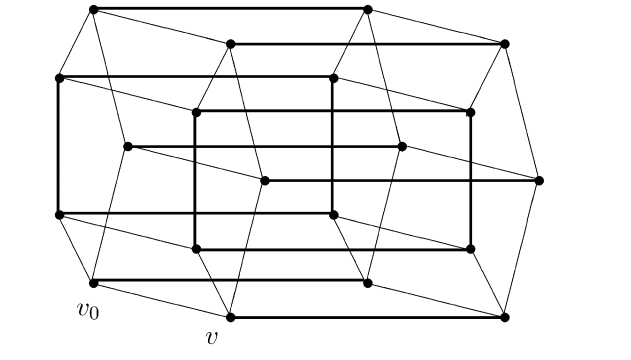
\includegraphics[width = 10cm]{rys1.png}
\caption{G=$C_5 \square K_s \square K_2 = C_5 \square C_4$}
\end{figure}

\newpage
\subsection{Kolorowanie właściwe produktu iloczynu kartezjańskiego grafów}
Rozważmy dwa połączone wierzchołki $u$ oraz $v$ w grafie G. Ponieważ są połączone to ich współrzędne różnią się dokładnie na jednej pozycji. Niech $i$ oznacza tę pozycję. Wtedy krawędź $uv$ należy do $G_i^v$. Zdefiniujmy następującą funkcję $c$ na zbiorze krawędzi $G$. Niech $c(uv) = i$.\\
Podsumowując: funkcja $c: E(G) \rightarrow \{1,2,...,k\}$ jest kolorowaniem właściwym produktu iloczynu kartezjańskiego, jeżeli $c(uv) = i $ wtedy i tylko wtedy gdy współrzędne wierzchołków $u$ oraz $v$ różnią się na $i$-tej pozycji.\\
Każda krawędź należy dokładnie do jednej warstwy. Rozważając podgraf grafu $G$ składający się z krawędzi koloru $i$ to każda spójna składowa tego podgrafu będzie oddzielną i-tą warstwą grafu $G$.
\subsection{Lemat o trójkącie}
\textit{\textbf{Twierdzenie:} Niech $G$ będzie produktem kartezjańskim grafów $G_1, G_2, ... , G_k$ oraz $c: E(G) \rightarrow \{1,2,...,k\}$ kolorowaniem właściwym produktu iloczynu kartezjańskiego. Wówczas każdy trójkąt w grafie $G$ jest monochromatyczny.}\\
\\
\textit{\textbf{Dowód}}\\
Niech wierzchołki $v_1, v_2, v_3$ będą parami sąsiednie. Załóżmy, nie wprost, że $i=c(v_1 v_2 ) \neq c(v_2 v_3)=j$. Wówczas współrzędne wierzchołków $v_1$ i $v_2$ różnią się na $i$-tej pozycji natomiast $v_2$ i $v_3$ na $j$-tej pozycji. Tak więc współrzędne $v_1$ oraz $v_3$ różnią się na pozycjach $i$-tej oraz $j$-tej, W takim razie wierzchołki te nie mogą być ze sobą połączone. A więc dochodzimy do sprzeczność.\\
Na podstawie powyższego lematu stwierdzamy, że każdy kwadrat zawierający co najmniej jedną przekątną jest tego samego koloru.\\
\subsection{Lemat o kwadracie}
\textit{\textbf{Twierdzenie:} Niech $c: E(G) \rightarrow {1,2,...,k}$ będzie właściwym kolorowaniem grafu $G$ będącego produktem kartezjańskim. Dane są dwie połączone krawędzie $e$ i $f$ różnych kolorów. Wówczas istnieje dokładnie jeden kwadrat bez przekątnych (graf $C_4$) zawierający $e$ oraz $f$.}\\
\\
\textit{\textbf{Dowód:}}\\
Przyjmijmy następujące oznaczenia:\\
$v$- wspólny wierzchołek krawędzi $e$ oraz $f$, $v_e$- drugi koniec $e$, $v_f$- drugi koniec $f$\\
$(v_0 , v_1, ... ,v_i, ..., v_j,...,v_k )$- współrzędne wierzchołka $v$\\
$(v_0 , v_1, ... ,v'_i, ..., v_j,...,v_k )$- współrzędne wierzchołka $v_e$\\
$(v_0 , v_1, ... ,v_i, ..., v'_j,...,v_k )$- współrzędnymi wierzchołka $v_f$\\
$v'$- wierzchołek o współrzędnych $(v_0 , v_1, ... ,v_i', ..., v'_j,...,v_k )$\\ 
\\
Łatwo stwierdzić, że wierzchołek $v'$ jest połączony z wierzchołkiem $v_e$ ponieważ ich współrzędne różnią się tylko na pozycji $j$ oraz w grafie $G_j$ istnieje krawędź $v_j v'_j$ ponieważ w grafie $G$ istnieje krawędź $f$. Analogicznie stwierdzamy istnienie krawędzi $v'v_f$, co w połączeniu z faktem, że krawędzie $e$ oraz $f$ są różnego koloru i rozważaniom na temat kwadratów z przekątnymi daje nam tezę lematu. Co więcej na podstawie powyższego rozumowania, można wnioskować że przeciwległe krawędzie w kwadracie mają ten sam kolor, niezależnie czy kwadrat posiada przekątne czy też nie.\\

\subsection{Lemat o izomorfizmie}
\textit{\textbf{Twierdzenie: }Niech $G=(V, E)$ będzie spójnym grafem, natomiast $E_1 , E_2 , ... , E_k$ podziałem zbioru krawędzi. Niech każda spójna składowa $(V, \cup_{j \neq i}E_j)$ ma dokładnie jeden punkt wspólny z każdą spójną składową $(V, E_i)$ oraz krawędzie między dwoma składowymi $(V, E_i)$ wyznaczają izomorfizm między tymi składowymi (jeżeli takie krawędzie istnieją). Wtedy: $G=\Pi G_i $ gdzie $G_i $ jest dowolną, spójną składową $(V, E_i)$.}\\
\\
Graf spełnia założenia izomorfizmu, jeżeli spełnia założenia lematu o izomorfizmie. \\
Niech dwie spójne składowe $C$ i $D$ grafu $(V, E_i)$ będą sąsiednie. Aby sprawdzić czy krawędzie między tymi warstwami indukują izomorfizm wystarczy sprawdzić czy każda krawędź z $C$ i $D$ jest zawarta w jednym kwadracie zawierającym po jednej krawędzi z $C$ i $D$ a dwie pozostałe krawędzie to krawędzie między tymi składowymi. Procedura ta jest podobna jak szukanie kwadratu w poprzednim podrozdziale. Wnioski te będą używane podczas procedury zwanej sprawdzaniem spójności.\\
\\
Podrozdział ten zakończymy pewnym sformułowaniem. Generalnie, w naszym algorytmie, nie będziemy opisywać procedury dzielenia krawędzi na podzbiory, lecz wykonywać będziemy procedurę kolorowania. Oczywiście łatwo można stwierdzić, że będą to dla nas procedury równoważne, aczkolwiek nie będziemy już o tym wspominać, tylko korzystać z tego faktu, głównie we wspomnianej już wcześniej procedurze sprawdzania spójności.\\ 
\subsection{Lemat o udoskonaleniu faktoryzacji iloczynu kartezjańskiego}
\textit{\textbf{Twierdzenie:} Faktoryzacja prosta danego grafu spójnego jest taka sama lub lepsza niż każda inna faktoryzacja tegoż grafu.}\\
\\
Dowód tego twierdzenia wynika wprost z faktu, że każdy graf spójny podsiada jednoznaczną faktoryzację prostą. \\
\\
Lemat ten będzie przez nas wykorzystywany w procedurze łączenia kolorów. W algorytmie opisanym w ostatnim rozdziale zakładamy, że faktoryzacja grafu wejściowego będzie się składać z pewnej, oszacowanej przez nas z góry, liczby czynników, co daje nam pewność że uzyskana przez nas finalna faktoryzacją będzie faktoryzacją pierwszą.
\newpage
\section{Faktoryzacja z dodatkowymi informacjami}
W tym rozdziale przedstawimy algorytm kolorowania właściwego grafu względem iloczynu kartezjańskiego, mając podane kolory krawędzi wychodzących z pewnego wierzchołka, względem danego rozkładu grafu. Następnie pokażemy jak mając kolory wszystkich krawędzi nadać współrzędne wierzchołkom. 
\\
\subsection{Algorytm kolorowania krawędzi}
Załóżmy, że mamy dane kolory wszystkich krawędzi, w kolorowaniu iloczynu kartezjańskiego grafu, wychodzących z pewnego wierzchołka $v_0$. Kolorowanie pozostałych krawędzi będzie odbywało się w kolejności przeszukiwania grafu w algorytmie BFS z wierzchołkiem początkowym $v_0$. \\
\\
\textit{\textbf{Twierdzenie 3.1:} Niech G=$G_1 \square G_2 \square ... \square G_k$ będzie grafem spójnym. Dane jest kolorowanie właściwe względem podanego rozkładu dla wszystkich krawędzi wychodzących z pewnego wierzchołka $v_0$. Wtedy kolorowanie właściwe produktu kartezjańskiego może być uzyskane zgodnie z kolejnością algorytmu BFS o wierzchołku początkowym $v_0$. Złożoność czasowa tego algorytmu to $\mathcal{O}(mn)$, natomiast złożoność pamięciowa $\mathcal{O}(n^2)$}.\\
\\
\textit{\textbf{Dowód}}\\
Jako dowód przedstawiony zostanie algorytm kolorowania krawędzi. W pierwszym kroku algorytmu dzielimy zbiór wierzchołków grafu $G$ na podzbiory $L_0 , L_1, L_2 , ..., L_r$ w taki sposób, że wierzchołek $v$ należy do zbioru $L_i$ wtedy i tylko wtedy gdy odległość wierzchołka $v$ od wierzchołka $v_0$ jest równa $i$. Zbiory te będziemy nazywać poziomami. Następnie dla każdego wierzchołka, wszystkie krawędzie incydentne z tym wierzchołkiem dzielimy na trzy zbiory- zbiór krawędzi dolnych, poprzecznych i górnych. Definiowanie tych zbirów przebiega następująco. Rozważy poziom $i$, następnie dla wszystkich wierzchołków $v$ należących do zbioru $L_i$ rozważamy krawędzie $vu$ incydentne z $v$. Wówczas jeżeli $u$ należy do $L_{i-1}$ to krawędź $vu$ będzie krawędzią dolną. Jeżeli $u$ należy do $L_i$ wówczas $uv$ będzie krawędzią poprzeczną, jeżeli natomiast $u$ należy do $L_{i+1}$ wówczas $uv$ będzie krawędzią górną wierzchołka warstwy $L_i$. Zauważmy, że krawędzie dolne wierzchołków poziomu $L_{i+1}$ są krawędziami górnymi wierzchołków poziomu $L_{i}$ .\\
\\
Nasz algorytm rozpoczynamy od pokolorowania krawędzi poprzecznych $L_1$. Nie stanowi to problemy, ponieważ każdy trójkąt jest monochromatyczny. Tak więc każdej krawędzi $uv$ nadajemy kolor krawędzi $v_0 v$ czyli $c(uv):=c(v v_0 )=c(u v_0 )$.\\
\\
Następnie indukcyjnie kolorujemy krawędzie dolne a następnie poprzeczne $L_{i+1}$ mając już pokolorowane krawędzie dolne i poprzeczne $L_i$. Nie ma potrzeby kolorowania krawędzi górnych $L_i$ ponieważ zbiór ten jest również zbiorem krawędzi dolnych $L_{i+1}$.\\
\\
Zaczynamy od krawędzi dolnych. Przeglądamy wierzchołki należące do $L_{i+1}$ zgodnie z kolejnością wyznaczoną przez algorytm BFS. Niech dany będzie wierzchołek $u$ oraz krawędź $uv$. Ponieważ wierzchołek v należy do $L_i$, gdzie $i\geqslant 1$ to istnieje wierzchołek $w$ należący do $L_{i-1}$ sąsiedni z $v$. Rozważmy dwa przypadki:
\begin{enumerate}
\item Nie istnieje wspólny sąsiad wierzchołków $u$ oraz $w$ różny od $v$. Wówczas nie istnieje kwadrat zawierający wierzchołki $u$ oraz $w$ a co za tym idzie kolory krawędzi $uv$ oraz $vw$ są te same czyli $c(uv):=c(vw)$.
\item Istnieje wspólny sąsiad $x$ wierzchołków $u$ oraz $w$ różny od $v$. W tym przypadku $c(uv):=c(xw)$ oraz $c(ux):=c(vw)$. 
\end{enumerate}
Uzasadnienia w obydwu przypadkach wynikają z lematu o kwadracie.\\
Rozważmy teraz krawędzie poprzeczne $L_{i+1}$. W tym celu również przeglądamy wierzchołki należące do tego poziomu. Dla każdej krawędzi $uv$ należącej do krawędzi poprzecznych rozważanego poziomu szukamy krawędzi dolnej $uw$ i podobnie jak dla krawędzi dolnych szukamy wspólnego sąsiada wierzchołków $v$ oraz $w$. Jeśli takowy wierzchołek $x$ istnieje wówczas $c(uv):=c(wx)$, jesli nie $c(uv):=c(uw)$.\\
\\
Zauważmy, że aby wyznaczyć $G_i$ wystarczy znaleźć $G_i ^{v_0}$. Wierzchołek $v$ należy do $V(G_i ^{v_0})$ wtedy i tylko wtedy gdy wszystkie jego krawędzie dolne są koloru $i$. Tak więc aby wyznaczyć $G_i$ wystarczy przejrzeć wszystkie krawędzie dolne wszystkich wierzchołków, jeżeli lista ta jest monochromatyczna wierzchołek ten będzie należał do $V(G_i ^{v_0})$ gdzie $i$ to kolor krawędzi dolnych tego wierzchołka.\\
Rozważając jeszcze raz krawędzie dolne oraz poprzeczne wierzchołków warstw jednostkowych, na podstawie spójności produktu iloczynu kartezjańskiego stwierdzamy, że i krawędzie dolne i krawędzie poprzeczne tychże wierzchołków należą do warstw jednostkowych.\\
\\
Na koniec pozostaje nam wykazanie, że nasz algorytm rzeczywiście spełnia założenia dotyczące złożoności pamięciowej i czasowej. Zauważmy że dla każdego wierzchołka należącego do $L_i$, gdzie $i>0$ szukamy dolnego sąsiada, następnie przeglądamy wszystkie krawędzie dolne oraz poprzeczne. Tak więc wykonujemy co najwyżej $2m$ kroków w naszym algorytmie, gdzie $m$ oznacza liczbę krawędzi naszego grafu $G$. Dla ustalonych krawędzi $uv$ oraz $uw$ szukamy wspólnego sąsiada $x$. Mamy co najwyżej $n=G(V)$ możliwości wyboru tego sąsiada. Jeżeli informacje o krawędziach grafu są przetrzymywane w tablicy sąsiedztwa sprawdzenie czy dany wierzchołek jest sąsiadem innego można wykonać w czasie stałym. Tak więc dowiedliśmy, że złożoność czasowa algorytmu to $\mathcal{O}(mn)$. Natomiast złożoność pamięciowa $\mathcal{O}(n^2)$. Zauważmy, że jedyną strukturą danych, którą stworzyliśmy w czasie działania programu są tablice krawędzi dolnych, poprzecznych i górnych. Tak więc całkowity rozmiar tych tablic będzie wynosił $2m$, ponieważ każda krawędź trafi dokładnie do dwóch tablic. Porównując to z wejściowymi strukturami danych, nasza złożoność pamięciowa nie wzrosła, gdyż jest ona ograniczona z góry przez $\mathcal{O}(n^2)$, czyli rozmiar tablicy sąsiedztwa naszego grafu wejściowego. \\
\subsection{Nadawanie współrzędnych wierzchołkom}
W poprzednim podrozdziale opisaliśmy algorytm kolorowania krawędzi, jednakże nie podawaliśmy sposobu, jak nadać współrzędne wierzchołkom. Zdefiniujemy teraz algorytm, który nada współrzędne naszym wierzchołkom, mając już dane kolory wszystkich krawędzi.\\
\\
\textit{\textbf{Twierdzenie 3.2:} Niech G=$G_1 \square G_2 \square ... \square G_k$ będzie grafem spójnym. Dane jest również kolorowanie właściwe produktu względem podanego rozkładu. Algorytm nadania współrzędnych wierzchołkom może być zrealizowany w złożoności czasowej i pamięciowej $\mathcal{O}(m)$.}\\
\\
\textit{\textbf{Dowód}}\\
Na początku dokonajmy małej obserwacji. Liczba czynników w rozkładzie względem iloczynu kartezjańskiego jest co najwyżej równa minimalnemu stopniowi w gragie wejśiowym $G$. Aby to umotywować wystarczy wspomnieć, że każdy wierzchołek $v$ należy do każdej z warstw $G_1, G_2, ..., G_k$, a co za tym idzie z tego wierzchołka wychodzi co najmniej jedna krawędź każdego koloru. To rozważanie można oczywiście zastosować również do wierzchołka o minimalnym stopniu.\\
Dla każdego wierzchołka, aby móc przechować informację o jego współrzędnych, potrzebujemy $k$- elementowej tablicy. Ponieważ $k$ jest mniejsze od minimalnego stopnia grafu $d_0$ oraz $d_0 \cdot n \leqslant m$ to całkowity rozmiar tablic ze współrzędnymi spełnia nasze założenie o złożoności pamięciowej naszego algorytmu.\\
Algorytm rozpoczynamy od nadania wierzchołkowi $v_0$ współrzędnych składających się z samych 0. Następnie przeszukujemy wszystkie wierzchołki zgodnie z kolejnością algorytmu BFS. \\Jeżeli wierzchołek należy do $i$-tej warstwy jednostkowej jego wszystkie współrzędne otrzymują wartość 0 z wyłączeniem $i$-tej współrzędnej. Przeszukując wierzchołki $i$-tej warstwy jednostkowej $i$-tej współrzędnej nadajemy kolejną liczbę naturalną. Zapisując formalnie jeżeli nasz wierzchołek $u$ należy do warstwy jednostkowej $u_j =0$ dla $j \neq i$
oraz $u_i = max\{v_i\}+1$ gdzie $v_i $ to $i$-te współrzędne wierzchołków należących do $G_i$, odwiedzonych wcześniej niż wierzchołek $u$ w algorytmie BFS. 
Jeżeli natomiast wierzchołek nie należy do warstwy jednostkowej to istnieją co najmniej dwie krawędzie dolne tego wierzchołka, mające różne kolory. Niech tym wierzchołkiem będzie $u$ natomiast jego krawędziami dolnymi $uv$ oraz $uw$. Wówczas $u_i = max(v_i , w_i )$ dla $1 \leqslant i \leqslant k$. Tak więc dla pojedynczego wierzchołka wykonamy $k$ operacji, i w zestawieniu z obserwacją na początku tego dowodu, stwierdzamy, że nasza zakładana złożoność obliczeniowa została osiągniętą.
\newpage
\section{Etykietowanie produktu kartezjańskiego}
W tym rozdziale rozszerzymy definicję kolorowania i nazwiemy ją etykietowaniem. Wszystkie krawędzie, rzutowane na tą samą krawędź otrzymają tę samą etykietę. Pokażemy, że produkt może być poetykietowany, a co za tym idzie pokolorowany w czasie liniowym. Etykietowanie pozwoli nam na określenie pozycji danej krawędzi w stosunku do faktoryzacji iloczynu kartezjańskiego grafu w czasie stałym. W rozdziale tym opiszemy struktury danych niezbędne do etykietowania krawędzi. Patrząc z punktu widzenia algorytmu, etykietowanie jest pozycją krawędzi w tablicy krawędzi wychodzących z danego wierzchołka o tym samym kolorze. \\
\subsection{Struktury Danych}
Zauważmy, że używamy współrzędnych wierzchołka do określenia jego pozycji w produkcie iloczynu kartezjańskiego. Całkowita długość tych wektorów jest równa $O(m)$. Przez pozycję krawędzi $uv$ rozumiemy pozycję wierzchołka $u$, kolor krawędzi $uv$ oraz rzutowanie $p_i (uv)$, czyli $p_i(u) p_i(v)$. Krawędź $p_i (uv)$ będziemy nazywać bazą krawędzi $uv$. \\
Krawędź $uv$ ma ten sam kolor co krawędź $p_i (u)p_i(v)$ oraz tak samo jest krawędzią dolną, poprzeczną lub górną. Poniżej przedstawimy jak efektywnie przetrzymywać informację o bazie. \\
W poprzednich rozdziałach opisywaliśmy w jaki sposób dzielimy krawędzie incydentne z danym wierzchołkiem na krawędzie dolne, poprzeczne i górne. Następnie każdą taką listę można podzielić na krawędzie tego samego koloru. Pozycja krawędzi, w tak stworzonej monochromatycznej liście, posłuży nam do zlokalizowania $p_i(uv)$, będziemy ją nazywać numerem danej krawędzi i oznaczać $n(uv)$. W ogólnym przypadku $n(uv) \neq n(vu)$. Parę $<c(uv), n(uv)>$ będziemy nazywać etykietą $uv$ i oznaczać $l(uv)$. Razem z $p_{c(uv)}(u)$ będzie ona opisywać pozycję krawędzi w produkcie. \\
Ilość tablic monochromatycznych będzie równa co najwyżej $3d(v_0 )$ dla każdego wierzchołka (po $d(v_0)$ dla krawędzi dolnych, poprzecznych i górnych), tak więc dostęp do tych tablic może odbyć się w czasie stałym.\\
Tak więc etykietowanie zostało zdefiniowane. Jak się okaże, będzie ono zależne tylko od kolejności krawędzi należących do warstw jednostkowych oraz krawędzi górnych należących do wierzchołków z warstw jednostkowych. Kolejność pozostałych krawędzi, podana na wejściu, nie będzie miała wpływu na rezultat etykietowania,co więcej naszym celem będzie ustalenie tej kolejności. \\
W algorytmie dobrze uwzględnić że krawędź dolna, poprzeczna lub górna $uv$ ma początek w $u$ natomiast koniec w $v$. Pozwoli to na znalezienie tej krawędzi w liście monochromatycznej w czasie stałym, jeżeli znamy jej numer. W tym celu zmodyfikujemy również macierz sąsiedztwa tak, aby w komórce $uv$ mieć numer danej krawędzi aby znalezienie jej numeru mogło się dobyć w czasie stałym. \\
Podsumowując, w naszym algorytmie będziemy używać następujących struktur danych: dla każdego wierzchołka lista sąsiedztwa oraz zmodyfikowaną tablicę sąsiedztwa całego grafu. Dodatkowo każdy wierzchołek zostanie ułożony w tablicy zgodnie z kolejnością algorytmu BFS, będzie on posiadał numer swojego poziomu, wektor współrzędnych (o długości nie większej niż $d(v_0)$) oraz listę krawędzi dolnych, poprzecznych oraz górnych, które następnie będą dzielone na listy monochromatyczne. Budowa tychże struktur, z wyłączeniem list monochromatycznych jest możliwa w czasie $O(m)$. Pokażemy, że i te tablice można zbudować w takim czasie. W następnym rozdziale pokażemy również, jak zastąpić tablicę sąsiedztwa aby nasza złożoność pamięciowa uległa poprawie. \\
\\
\subsection{Algorytm Etykietowania}
\textit{\textbf{Twierdzenie 4.2:} Niech G=$G_1 \square G_2 \square ... \square G_k$ będzie grafem spójnym. Dane jest również kolorowanie właściwe produktu względem podanego rozkładu dla krawędzi wychodzących z wierzchołka $v_0$. Etykietowanie tego grafu może być zrobione w czasie O(m)}\\
\\
\textit{\textbf{Dowód}}\\
Opiszemy liniowy algorytm etykietowania. Poetykietowanie krawędzi wychodzących z $v_0$ nie stanowi problemu. Następnie etykietujemy krawędzie dolne i poprzeczne wierzchołków należących do warstwy $L_1$. To również nie stanowi problemu ponieważ wszystkie krawędzie dolne dostają numer $1$ natomiast krawędzie poprzeczne kolorujemy tak jak w rozdziale 3, numery tych krawędzi są zgodne z kolejnością w jakiej zostały podane na wejściu. \\
Zakładamy, że mamy poetykietowane krawędzie dolne i poprzeczne dla warstwy $L_i$ oraz górne warstwy $L_{i-1}$ i indukcyjnie etykietujemy krawędzie dolne i poprzeczne warstwy $L_{i+1}$ oraz górne warstwy $L_i$. Niech wierzchołek $u$ należy do warstwy $L_{i+1}$. Zacznijmy od krawędzi dolnych. \\
\begin{enumerate}
\item Wierzchołek ma tylko jedną krawędź dolną. Wówczas kolorujemy tak, jak to było w rozdziale 3.1 natomiast krawędź otrzymuje numer $1$. 
\item Szukamy kwadratu bazowego dla wierzchołków posiadających więcej niż jedną krawędź dolną. \\
Niech $uv$ będzie pierwszą taką krawędzią. Natomiast niech $vx$ będzie krawędzią dolną wierzchołka $v$. Szukamy wspólnego sąsiada wierzchołków $u$ oraz $x$ różnego oczywiście od wierzchołka $v$. Znalezienie tego sąsiada odbywa się z użyciem tablicy sąsiedztwa i porównaniu sąsiadów. Złożoność czasowa tej operacji to $\mathcal{O}(d(u))$.\\
\begin{enumerate}[a)]
\item
Jeżeli wspólny sąsiad nie istnieje, wówczas $c(uv):=c(vx)$. Pozostałe krawędzie dolne również kolorujemy tym samym kolorem. Oznacza to, że wierzchołek $u$ należy do warstwy jednostkowej, a co za tym idzie możemy ponumerować krawędzie zgodnie z tym, w jaki sposób podano je na wejściu.\\
\item
Tak więc rozważmy przypadek, że istnieje wierzchołek $w$ będący wspólnym sąsiadem wierzchołków $u$ oraz $x$. Jeżeli kolory krawędzi $vx$ oraz $xw$ są różne wówczas $l(uv):=l(wx)$ oraz $l(uw):=l(vx)$. Inicjalizacja tablic monochromatycznych dla dolnych krawędzi wierzchołka $u$ również nie stanowi dla nas problemu. Wystarczy zauważyć, że, dla wierzchołka $u$, każda tablica, reprezentująca kolor różny od $c(uv)$ ma taką samą długość jak tablica dla wierzchołka $v$, natomiast tablica dla koloru $c(uv)$ będzie miała taką samą długość jak dla wierzchołka $w$. Samo etykietowanie tej krawędzi zostało wykonane w czasie stałym, dzięki modyfikacji tablicy sąsiedztwa, inicjalizacja tablic może być zrobiona w czasie $\mathcal{O}(d(v_0))$. Kwadrat $uvxw$ będziemy odtąd nazywać kwadratem bazowym i posłuży on nam do poetykietowania pozostałych dolnych krawędzi wierzchołka $u$.
\item
Zostaje do rozważenia przypadek, gdy kolory krawędzi $wx$ oraz $vx$ są takie same, a co za tym idzie, krawędzie $uw$ oraz $uv$ będą miały ten sam kolor. Jeżeli wszystkie pozostałe krawędzie dolne wierzchołka $v$ mają ten sam kolor wówczas wierzchołek $u$ należy do warstwy jednostkowej i postępujemy analogicznie jak w przypadku 2a. Tak więc niech istnieje krawędź $vx'$, której kolor różni się od koloru $vx$ a co za tym idzie również od $uv$. Tak więc musi istnieć wspólny sąsiad wierzchołków $u$ oraz $x'$ różny od $v$, nazwijmy go $w'$. Znalezienie takiego sąsiada może być wykonane w czasie $O(d(u))$. Dalej postępujemy jak w przypadku 2b a naszym kwadratem bazowym będzie $uvx'w'$.
\end{enumerate} 
\item
Etykietowanie pozostałych krawędzi dolnych odbywa się z udziałem znalezionego wcześniej kwadratu bazowego. Załóżmy dla jasności sytuacji, że kwadrat ten składa się z wierzchołków $u,v,x$ oraz $w$. Tak więc iterujemy po wszystkich krawędziach dolnych wierzchołka $u$. Niech $uy$ będzie kolejną taką krawędzią. Dalej niech $yz$ będzie dolną krawędzią wierzchołka $y$, taką, że $l(yz)=l(uv)$. Jeżeli okaże się że taka krawędź nie istnieje wówczas szukamy krawędzi $yz$ takiej, że $l(yz)=l(uw)$. Dla każdego wierzchołka taka operacja jest wykonywana w czasie stałym, a dla wszystkich krawędzi sumarycznie czas potrzebny do poetykietowania krawędzi dolnych jest równy $O(d(u))$. \\
\end{enumerate}
Tak więc etykietowanie krawędzi incydentnych z wierzchołkiem$u$ może być wykonane w złożoności czasowej $\mathcal{O}(d(u) + d(v_0))$ co sprowadza się do $\mathcal{O}(d(u)) $. Suma ta wynika z następujących operacji: dwukrotne wyszukiwanie wspólnego sąsiada, inicjalizacja tablic monochromatycznych oraz etykietowanie poszczególnych krawędzi.
Etykietowanie krawędzi górnych warstwy $L_i$ oraz poprzecznych warstwy $L_{i+1}$ przebiega w analogiczny sposób, więc i złożoność tych operacji jest taka sama.\\
Pozostaje sprawdzić złożoność czasową całej operacji, można ją opisać jako \\
$\mathcal{O}(\sum _{u \in V(G)} d(u)) = \mathcal{O}(m)$.\\
Jeżeli chodzi o złożoność pamięciową, to używaliśmy struktur opisanych w rozdziale 4.1 tak więc, nie licząc tablicy sąsiedztwa, jest ona równa $\mathcal{O}(m)$. Jednak użycie tejże tablicy sprawia, że całościowa złożoność pamięciowa jest równa $\mathcal{O}(n^2)$, co jak się okaże za chwilę będzie można poprawić do satysfakcjonującej nas złożoności. Opiszmy najpierw jak tego dokonać.\\
\subsection{Inicjalizowanie częściowe tablicy}
W tym podrozdziale zajmiemy się następującym problemem. Chcemy utworzyć tablicę, która będzie wypełniona tylko we wskazanych na początku miejscach. Dokładnie, naszym zadaniem jest utworzenie tablicy o rozmiarze $n$, w której wypełnione będzie dokładnie $d$ elementów (niekoniecznie początkowych i niekoniecznie spójnych). Tak utworzona tablica, w czasie stałym, ma nam dać informację, czy dane pole, o podanym indeksie, zostało zainicjalizowane, i jeśli tak, wskazać jaka wartość kryje się pod tym indeksem.\\
Zaczynamy od inicjalizacji pustej tablicy. W tym momencie, pod każdym indeksem w tej tablicy znajdziemy przypadkową wartość. Dokładając nowy element do tablicy wciąż jednak nie mamy informacji, czy element ten jest podaną przez nas wartością, czy jest on od momentu inicjalizacji. Tak więc tworzymy dodatkowy stos, na którym odkładamy indeksy, które zostały przez nas zainicjalizowane. W tym momencie, mamy już informację, które elementy są przez nas dodane a które nie. Jednakże sprawdzenie czy, dany element został przez nas dodany wymaga złożoności czasowej $\mathcal{O}(n)$ w pesymistycznym przypadku. Potrzebna jest więc nam jeszcze jedna struktura. Tworzymy tablicę wskaźników o rozmiarze $n$. Na początku tablica ta zawiera przypadkowe wartości. W momencie dodawania nowego elementu do tablicy początkowej, najpierw umieszczamy indeks na stosie, a następnie dodajemy, do naszej drugiej tablicy, wskaźnik na nowo utworzony element na stosie. Operacja dodawania nowego elementu wykonywana jest w czasie stałym, dostęp do elementu również w takim czasie może być wykonany- sprawdzamy najpierw, czy w tablicy wskaźników element o podanym indeksie wskazuje na zmienną na naszym stosie- jeżeli nie, oznacza to, że nie inicjalizowaliśmy elementu o podanym indeksie. Jeżeli tak, w prosty sposób pobieramy wartość z naszej tablicy początkowej.\\
Złożoność pamięciowa naszej operacji to $\mathcal{O}(n)$, gdyż mamy trzy struktury o takiej samej złożoności- tablicę początkową, stos, oraz tablicę wskaźników. Złożoność pamięciowa tej operacji to $\mathcal{O}(d)$, gdzie $d$ oznacza ilość inicjalizowancyh elementów.\\

\subsection{Etykietowanie produktu w czasie liniowym}
Dotychczas do sprawdzenia czy dwa wierzchołki są połączone używaliśmy macierzy sąsiedztwa, co wymagało od nas użycia $\mathcal{O}(n^2)$ pamięci, gdzie $n$ oznacza liczbę wierzchołków. Zaburza to nasze założenie o liniowej złożoności pamięciowej naszego algorytmu, co więcej inicjalizacja tej macierzy również może zaburzyć naszą złożoność czasową. Zauważmy jednak, że w każdym kroku naszego algorytmu potrzebujemy co najwyżej jednego wiersza z naszej tabeli sąsiedztwa. A ponieważ nasz graf jest spójny, czyli posiada co najmniej $n-1$ krawędzi, wiersz z macierzy sąsiedztwa nie zaburzy naszej złożoności pamięciowej. Pozostaje problem jak zainicjalizować nasz wiersz w taki sposób, aby sumaryczna inicjalizacja wszystkich wierszy nie zwiększyła złożoności czasowej z $O(m)$ do $O(n^2)$. W tym celu posłużymy się rozwiązaniem zaproponowanym w poprzednim podrozdziale.\\
Wykorzystując tę metodę, do tworzenia wiersza tablicy sąsiedztwa, zauważmy na początek, że czas potrzebny do stworzenia takiego wiersza dla wierzchołka $x$ jest proporcjonalny do $d(x)$. A ponieważ $\sum_{v \in V(G)}d(v) = 2m$ to złożoność czasowa potrzebna na wykonanie się algorytmu nie zmieni się, dopóki nie będziemy wykonywać naszej operacji więcej niż stałą ilość razy dla poszczególnych wierzchołków. Tak więc w tym podrozdziale opiszemy jak wykonać nasz algorytm tak, aby nasze założenie zostało wykonane, co pozwoli nam na utrzymanie złożoności czasowej, przy jednoczesnym zmniejszeniu złożoności pamięciowej.\\
\\
\textit{\textbf{Twierdzenie} Niech G=$G_1 \square G_2 \square ... \square G_k$ będzie grafem spójnym. Dane jest również kolorowanie właściwe produktu względem podanego rozkładu dla krawędzi wychodzących z wierzchołka $v_0$. Złożoność czasowa i pamięciowa tego algorytmu wynosi O(m)}.\\
\\
\textit{\textbf{Dowód}}\\ 
W rozdziale 4.2 opisaliśmy liniowy, jeżeli chodzi o złożoność czasową algorytm, tutaj opiszemy jak go zmodyfikować aby i złożoność pamięciowa była liniowa. Opiszemy modyfikację trzech kroków z poprzedniego rozdziału.\\
\begin{enumerate}
\item 
Jeżeli chodzi o etykietowanie krawędzi dolnych wierzchołków posiadających jedną krawędź dolną procedura się nie zmienia.
\item
Poszukiwanie kwadratu bazowego. Możliwe, że będą konieczne dwa przebiegi poszukiwań naszego kwadratu bazowego. W pierwszym przebiegu wierzchołek $v$ jest dolnym wierzchołkiem $u$, gdzie $u \in L_{i+1}$ natomiast $x$ jest dolnym wierzchołkiem $v$. Teraz szukamy pozostałych wierzchołków $u'$ należących do warstwy $L_{i+1}$, dla których odległość od wierzchołka $x$ również wynosi 2. Dopiero wtedy będziemy tworzyć wiersz macierzy sąsiedztwa wierzchołka $x$. W drugim przebiegu rozumowanie jest analogiczne. 
\item
W tym fragmencie konieczne będzie tworzenie wiersza macierzy sąsiedztwa maksymalnie dwa razy, tym razem jednak dla wierzchołków należących do warstwy $L_i$, a nie jak to było w punkcie 2 dla warstwy $L_{i-1}$.
\end{enumerate}
Dla krawędzi górnych i poprzecznych procedura wygląda analogicznie (możliwe, że konieczne będą po dwa przebiegi kroku algorytmu). Tak więc podczas indukcyjnego kroku dla warstwy $L_{i+1}$ maksymalnie 4 razy szukamy wiersza macierzy sąsiedztwa dla wierzchołków warstw $L_{i} $ oraz $L_{i-1}$ co oznacza, że dla danego wierzchołka, jego wiersz z macierzy sąsiedztwa będzie wyszukiwany nie więcej niż 8 razy, co należało dowieźć. \\

Ponieważ etykietowanie jest rozszerzeniem kolorowania, nadanie współrzędnych wierzchołkom grafu $G$ może być wykonane przez algorytm opisany w rozdziale 3.2.\\
\newpage
\section{Sprawdzanie spójnosci}
Poprzednie rozdziały opierały się na założeniach, że znamy kolory krawędzi wychodzących z pewnego wierzchołka. Następnie etykietowaliśmy pozostałe krawędzie. Odwróćmy teraz trochę sytuację i załóżmy, że mamy dane etykiety pewnych krawędzi wychodzących z danego wierzchołka a naszym zadaniem będzie sprawdzenie, czy dane etykietowanie jest etykietowaniem produktu iloczynu kartezjańskiego według pewnego rozkładu. Jak się okaże w następnym rozdziale, jeżeli podamy złe kolory dla krawędzi wychodzących z wierzchołka $v_0$ nasza procedura etykietowania, może się nie wykonać z pewnych przyczyn. Możliwe jest jednak, że wykona się ona bez problemu nawet, gdy podane kolory będą niepoprawne. W tym celu wracamy do lematu o izomorfiźmie. Naszym zadaniem będzie sprawdzenie, czy na danym etapie, założenia lematu o izomorfizmie, tak aby cały czas mieć pewność, że nasze kolorowanie może być kolorowaniem właściwym produktu iloczynu kartezjańskiego. Procedurę tę będziemy zwać sprawdzaniem spójności.\\
Izomorfizm grafów jest bijekcją na zbiorach wierzchołków zachowującą sąsiedztwo. Korzystając z kolejności wierzchołków grafu uzyskaną w algorytmie BFS, będziemy indukcyjnie sprawdzać czy dla danego poziomu $L_i$ nasze założenia są spełnione i dalej kontynuować sprawdzenie dla następnych poziomów. \\
\\
\textit{\textbf{Twierdzenie} Załóżmy, że własności izomorfizmu są zachowane dla wierzchołków warstw $L_1$ do $L_i$. Sprawdzenie czy własności izomorfizmu dla wierzchołków należących do warstwy $L_{i+1}$ może być wykonane w czasie proporcjonalnym do sumy ilości krawędzi dolnych i poprzecznych warstwy $L_{i+1}$ oraz krawędzi górnych $L_{i}$.} \\
\\
\textit{\textbf{Dowód}}\\
Nasze sprawdzenie zaczyamy od dwustopniowej procedury.\\
\begin{enumerate}
\item
Dla każdego wierzchołka $u$ należącego do $L_{i+1}$, który nie jest wierzchołkiem warstwy jednostkowej, wybieramy dwie krawędzie dolne różnych kolorów $uv$ oraz $uw$ (można wybrać krawędzie należące do kwadratu bazowego) i sprawdzamy czy krawędzie dolne/poprzeczne wierzchołka $u$ mają odpowiednika wśród krawędzi dolnych/poprzecznych wierzchołka $v$. Uściślając, dla każdej krawędzi dolnej/poprzecznej $uz$ koloru różnego od $c(uv)$ istnieje dokładnie jedna krawędź dolna/poprzeczna $vz'$ taka, że $l(uz)=l(vz')$ i vice versa. Co więcej $l(uv)=l(zz')$.
\item
Dla krawędzi górnych należących do $L_i$ postępujemy analogicznie. Iterujemy po wszystkich wierzchołkach. Jeżeli $u$ nie należy do warstwy jednostkowej wybieramy kwadrat bazowy $uvxw$ i dla wszystkich krawędzi górnych wierzchołka $u$ porównujemy je z krawędziami $uv$ lub $uw$ w zależności od koloru.\\
Jeżeli $u$ należy do warstwy jednostkowej, załóżmy $G^{v_0}_i$, wybieramy jeden wierzchołek $v$, będący dolnym sąsiadem $u$. Porównujemy wówczas krawędzie górne wierzchołków $u$ oraz $v$ o kolorach różnych od $i$. 
\end{enumerate}

Ponieważ sprawdzenie, czy istnieje odpowiadająca krawędź, odkąd mamy posortowane listy monochromatyczne, może być wykonane w czasie stałym, czas potrzebny do znalezienia odpowiadających krawędzi, dla danego wierzchołka $u$, jest proporcjonalny do $d(u)$ a co za tym idzie, sumaryczna ilość czasu jest proporcjonalna do rozmiaru grafu. Żadne dodatkowe struktury danych nie są potrzebne. \\
Tak więc sprawdzanie izomorfizmów między warstwami może być wykonane w zadowalającej nas złożoności czasowej i pamięciowej. Aby wykazać, że jest to produkt iloczynu kartezjańskiego potrzeba jeszcze sprawdzić pozostałe założenia lematu o izomorfiźmie. Rozważmy wierzchołek $a$ będący dolnym sąsiadem $u$, takim że $c(ua) \neq c(uv)$. Będziemy teraz rozważać izomorfizm między $G^u_i$ oraz $G^a_i$ indukowany między krawędziami występującymi między tymi warstwami dla $i \neq c(uv)$.\\
Naszym zadaniem jest pokazanie, że dla każdej krawędzi dolnej lub poprzecznej $ab$, takiej że $c(ab) \neq c(ua)$ istnieje dokładnie jedna krawędź $uc$, taka że $l(uc)=l(ab)$ oraz wierzchołki $b$ i $c$ są połączone oraz $l(ua)=l(bc)$. Oczywiście do tego musimy pokazać również że dla każdej dolnej lub poprzecznej krawędzi $uc$ istnieje krawędź $ab$ spełniająca te same założenia.\\
Rozważmy pierwszy przypadek. We wcześniejszych rozważaniach w tym rozdziale wykazaliśmy istnienie krawędzi $aa'$, takiej że $l(uv)=l(aa')$. Z założenia indukcyjnego wiemy, że izomorfizmy są zachowane dla poziomów od $L_1$ do $L_i$. Skorzystamy teraz ponownie z lematu o kwadracie. Rozważając wierzchołki $a,b,a'$ w stałym czasie możemy znaleźć kwadrat $abb'a'$. Idąc dalej rozważamy wierzchołki $v,a',b'$ i również w czasie stałym możemy znaleźć kwadrat $va'b'c'$. Na koniec wystarczy rozważyć wierzchołki $b,b'c'$ i tak jak poprzednio w czasie stałym znajdujemy kwadrat $bb'c'c$. Krawędź $vc'$ posiada taką samą etykietę jak $ab$ oraz $cc'$ posiada taką samą etykietę jak $uv$. A ponieważ izomorfizm między wierzchołkami $v$ oraz $u$ został sprawdzony, wierzchołki $u$ oraz $c$ są połączone oraz etykiety $uc$ i $vc'$ są takie same, a co za tym idzie również etykieta $ab$ jest taka sama, udowodniliśmy zakładaną tezę. Dowód w drugą stronę przebiega analogicznie.\\
Pozostaje jeszcze sprawdzenie czy złożoność czasowa i pamięciowa nie uległy pogorszeniu. Zaczynając od złożoności pamięciowej, widzimy, że nie używamy żadnych dodatkowych, złożonych struktur danych. Co do złożoności czasowej, zauważmy że sprawdzenie izomorfizmu dla danej krawędzi odbywa się w czasie stałym. Szukanie kwadratów opiera się na korzystaniu z już posortowanych monochromatycznych list, więc dostęp do nich odbywa się w czasie stałym. Tak więc sumaryczna złożoność czasowa sprawdzania spójności może być wykonana w czasie proporcjonalnym do rozmiaru grafu.\\
\newpage

\section{Faktoryzacja poprzez łączenie kolorów}
W tym rozdziale opiszemy wszystkie konieczne narzędzia potrzebne do faktoryzacji spójnego grafu $G$ na grafy proste, czyli takie które nie da się opisać jako iloczyn dwóch nietrywialnych grafów (przez graf trywialny rozumiemy graf $K_1$). Z lematu o udoskonaleniu chcemy znaleźć końcowy rozkład podanego na wejściu grafu $G$. Przez znalezienie rozkładu rozumiemy znalezienie finalnego kolorowania właściwego produktu iloczynu kartezjańskiego. Ma to być kolorowanie zachowujące izomorfizmy między warstwami tego samego koloru.\\
\\
\textit{\textbf{Twierdzenie} Faktoryzacja prosta grafu spójnego może być wykonana w czasie liniowym i w takiej samej złożoności pamięciowej}\\
\\
\textit{\textbf{Dowód:}} Jako dowód zaprezentujemy algorytm. Ideą naszego rozumowania będzie rozpoczęcie algorytmu ze wskazanym kolorowaniem początkowym krawędzi wychodzących z wierzchołka o minimalnym stopniu. Kolorowanie to nie będzie jeszcze tym, które będzie wskazywać na kolorowanie właściwe finalnego produktu kartezjańskiego, lecz w trakcie działania algorytmu będziemy łączyć dwa kolory w jeden jeżeli zajdzie taka konieczność. \\
Nasz algorytm w pierwszym kroku nadaje różne kolory wszystkim krawędzią wychodzącym z wierzchołka $v_0$, który to jest wierzchołkiem o minimalnym stopniu w naszym grafie wejściowym. Ponieważ każdy wierzchołek posiada krawędzie incydentne każdego koloru wiemy, że w naszym kolorowaniu finalnym nie będzie więcej kolorów. Użycie wierzchołka o minimalnym stopniu sprawia również, że nasza początkowa tablica kolorów ma możliwie najmniejszy rozmiar, a co bardziej istotne jej wielkość jest stałą. \\
Na początek uruchamiamy algorytm BFS z wierzchołkiem początkowym $v_0$, dzielimy wierzchołki na warstwy a krawędzie na krawędzie dolne, poprzeczne i górne. Następnie dla każdej warstwy wykonujemy etykietowanie a następnie sprawdzamy spójność. Może się okazać, że nasza procedura wykona się bez błędów i w taki oto sposób otrzymamy nasze kolorowanie końcowe produktu iloczynu kartezjańskiego, a co za tym idzie rozkład naszego grafu wyjściowego na iloczyn grafów prostych.\\
Bardziej prawdopodobne jest jednak, że etykietowanie lub sprawdzanie spójności nie wykona się poprawnie. Dla przykładu, będziemy kolorować krawędzie poprzeczne warstwy $L_1$, widzimy wówczas, że nie jesteśmy w stanie pokolorować w takiej krawędzi (patrz lemat o trójkącie). Oznacza to po prostu, że nasze kolorowanie początkowe krawędzi wychodzących z $v_0$ jest niewłaściwe, użyliśmy zbyt dużej ilości kolorów. Wówczas procedura jest prosta- łączymy kolory krawędzi incydentnych z naszą krawędzią poprzeczną w jeden i wówczas możemy ją już pokolorować bez problemu. Cała idea naszego algorytmu opiera się na tym kopcenie: poetykietuj krawędzie i sprawdź spójność- jeżeli jest to niemożliwe- połącz kolory. \\
Jak się okazuje nie ma konieczności rekolorowania krawędzi, jeżeli już zostały pomalowane wcześniej, wystarczy tylko zanotować fakt, że dany kolor został połączony z innym. Ponieważ $d(v_0)^2 \leqslant d(v_0)n \leqslant 2m $ nie ma konieczności przetrzymywać danych o kolorach w żadnych skomplikowanych strukturach danych. Dodatkowo wiemy, że w finalnym kolorowaniu użyty będzie co najmniej jeden kolor, to operacji łączenia kolorów będzie również co najwyżej $d(v_0)$ co również nie zaburzy złożoności czasowej naszego algorytmu. W trakcie działania algorytmu kolory początkowe będziemy łączyć w zbiory połączonych kolorów. Kolor o najmniejszym indeksie w tablicy kolorów początkowych będziemy nazywać kolorem nominalnym i będzie on reprezentował zbiór kolorów połączonych w jeden. Te zbiory będziemy rozumieć jako nowe kolory. Tablice kolorów opisane w rozdziale o etykietowaniu będą zatem zawierać podtablicę kolorów początkowych i podziały będą tworzone właśnie według tych początkowych kolorów, oczywiście cały czas mając informację o tym czy i do jakiego koloru został dołączony dany kolor początkowy.\\
Generalnie krok naszego algorytmu będzie wyglądał następująco. Sprawdzamy spójność dla poziomu $L_i$. Następnie przechodzimy do etykietowania. Jeżeli nie będziemy mogli tego zrobić, oznacza to, że konieczne jest połączenie kolorów. Krótka analiza sprawia, że powody, dla których etykietowanie może nie zakończyć się sukcesem są następujące: zbyt mała liczba wierzchołków, zbyt mała liczba krawędzi lub przeciwnie zbyt duża liczba wierzchołków lub krawędzi. Może się również okazać, że algorytm, próbujący pobrać jakaś krawędź z list monochromatycznych nie będzie mógł tego zrobić ponieważ lista będzie za krótka. Analiza wykonana w pracy ~\cite{IMR} pozwoli nam dojść do wniosku, że etykietowanie nie wykona się poprawnie tylko w przypadku gdy rozważany wierzchołek należy do warstwy jednostkowej lub krawędź jest incydentna z takim wierzchołkiem. Oznacza to, że krawędzie dolne i poprzeczne incydentne z tym wierzchołkiem powinny być połączone w jedną listę monochromatyczną, o ile oczywiście łączymy kolory tych list w jeden. \\
Łatwo można stwierdzić, że nie ma potrzeby przekolorowania krawędzi z niższych warstw. Co więcej nie ma potrzeby jeszcze raz sprawdzania spójności. Wynika to z faktu, że mając mniej kolorów mamy mniej warstw, za to większych. A co za tym idzie, mamy mniej sprawdzania spójności między warstwami a sprawdzenia wykonane wcześniej dla krawędzi są wciąż ważne. \\
Następnie przechodzimy do sprawdzania spójności dla warstwy $L_{i+1}$. I podobnie jak dla etykietowania, jeżeli nie będziemy mogli przeprowadzić procedury z sukcesem, łączymy kolory. Podobnie jak dla etykietowania, stosując tę samą argumentację nie musimy sprawdzać niższych poziomów po połączeniu kolorów.\\ 


\begin{thebibliography}{99}
\bibitem{AUR} F. Aurenhammer, J. Hagauer, W. Imrich, 
Cartesian graph factorization at logarithmic cost per edge, Comput. Complexity 2 (1992) 331–349

\bibitem{FED} T. Feder, 
Product graph representations, J. Graph Theory 16 (1992) 467–488.

\bibitem{FEI} J. Feigenbaum, J. Hershberger, A.A. Schäffer, 
A polynomial time algorithm for finding the prime factors of Cartesian-product graphs, Discrete Appl. Math. 12 (1985) 123–138

\bibitem{MAIN} W. Imrich, I. Peterin, 
W. Imrich, I. Peterin / Discrete Mathematics 307 (2007) 472 – 483

\bibitem{IMR} W. Imrich, S. Klavžar, 
Product Graphs: Structure and Recognition, Wiley, New York, 2000

\bibitem{SAB} G. Sabidussi,
Graph multiplication, Math. Z. 72 (1960) 446–457.

\bibitem{VIS} V.G. Vizing,
The Cartesian product of graphs (Russian), Vycisl. Systemy 9 (1963) 30–43, English translation in Comput. Electron Syst. 2 (1966) 352–365.

\bibitem{VIS2} V.G. Vizing, 
Some unsolved problems in graph theory, Russian Math. Surveys 23 (1968) 125–141.

\bibitem{WIN} P.M. Winkler, 
Factoring a graph in polynomial time, European J. Combin. 8 (1987) 209–212
\end{thebibliography}
\end{document}
